S\-L\-I\-M Curve is a curve fitting library used for Fluorescent Lifetime Imaging or F\-L\-I\-M and Spectral Lifetime Imaging or S\-L\-I\-M. It is based on code developed by Paul Barber and the Advanced Technology Group at the Gray Institute for Radiation Oncology \& Biology, University of Oxford, and used for F\-L\-I\-M functionality in his T\-R\-I2 (Time Resolved Imaging) software. It is also used in the L\-O\-C\-I S\-L\-I\-M Plugin project.

For exponential lifetime fitting there are two core algorithms within S\-L\-I\-M Curve\-: The first is a triple integral method that does a very fast estimate of a single exponential lifetime component. The second is a Levenberg-\/\-Marquardt algorithm or L\-M\-A that uses an iterative, least-\/squares-\/minimization approach to generate a fit. This works with single, double and triple exponential models, as well as stretched exponential. There is also code to perform 'global' analysis over a number of signals symultaneously (e.\-g. over an image), where the lifetimes can be considered constant across the data set, but the amplitudes are allowed to vary for each signal. There is also a completely generic global analysis function. A third algorithm is available to perform phasor analysis.

In addition there is a non-\/negative linear least squares algorithm that is useful for spectral unmixing in S\-L\-I\-M.

The code is written in C89 compatible C and is thread safe for fitting multiple pixels concurrently. Several files are provided as wrappers to call this library from Java code\-: Ecf\-Wrapper.\-c and .h provide a subset of function calls used by S\-L\-I\-M Plugin, these may be invoked directly from Java using J\-N\-A. In addition there is a Java Curve\-Fitter project that provides a wrapper to the S\-L\-I\-M Curve code. This invokes the C code using J\-N\-I, with loci\-\_\-curvefitter\-\_\-\-S\-L\-I\-M\-Curve\-Fitter.\-c and .h.

For further details, see\-: \href{http://slim-curve.github.io/}{\tt http\-://slim-\/curve.\-github.\-io/}

If you are familiar with the program T\-R\-I2, that uses S\-L\-I\-M Curve, this screenshot may help you to understand the meaning of the parameters.

 
\begin{DoxyImage}
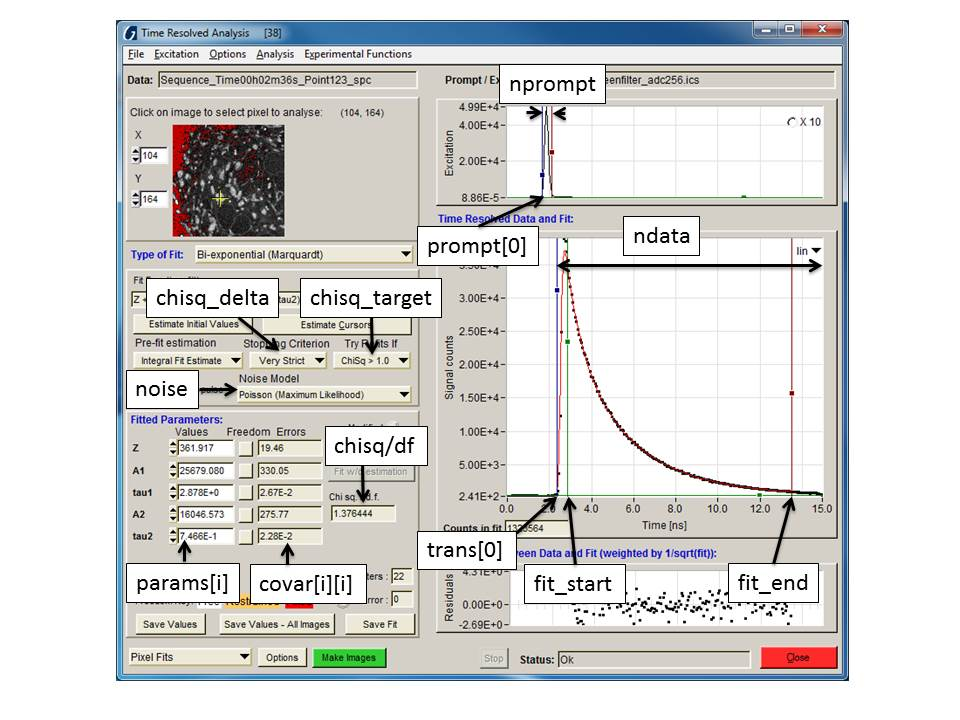
\includegraphics[width=15cm]{params_in_tri2.jpg}
\caption{How some S\-L\-I\-M-\/\-Curve paramters are used in T\-R\-I2.}
\end{DoxyImage}


\section*{Library Contents\-:}

\begin{TabularC}{2}
\hline
\rowcolor{lightgray}{\bf Directory }&{\bf Contents  }\\\cline{1-2}
src &source files \\\cline{1-2}
src/main/c &The source files for the S\-L\-I\-M Curve library \\\cline{1-2}
src/slim-\/curve-\/cmd/c &The source files for the stand alone executable wrapper for the library \\\cline{1-2}
test\-\_\-files &dat and ini settings file for testing \\\cline{1-2}
src/main/c/doc &A\-P\-I documentation (Doxygen output) \\\cline{1-2}
\end{TabularC}


\section*{To Build the Stand Alone Program using C\-Make and gcc under Linux\-:}

Create a build folder, and cd to it \begin{DoxyVerb}mkdir build
cd build
\end{DoxyVerb}


Run C\-Make \begin{DoxyVerb}cmake ../CMakeLists.txt
\end{DoxyVerb}


Run make \begin{DoxyVerb}make
\end{DoxyVerb}


\section*{To Run the Stand Alone Executable}

Copy the executable to the test\-\_\-files folder for convenience \begin{DoxyVerb}cp slim-curve-cmd ../test_files
\end{DoxyVerb}


Run the program with the test files \begin{DoxyVerb}cd ../test_files
./slim-curve-cmd test.ini transient.dat
\end{DoxyVerb}


\begin{DoxyAuthor}{Author}
Paul Barber 
\end{DoxyAuthor}
\begin{DoxyCopyright}{Copyright}
Creative Commons B\-Y-\/\-S\-A 2014 
\end{DoxyCopyright}
